%!TEX root = ../../../../memoria.tex
\subsection{Detalles de dirección}\label{chapter:solucionimplementada:section:address}

	Esta sección funciona exactamente igual \nameref{chapter:solucionimplementada:section:profile:subsection:book_address} ( \ref{chapter:solucionimplementada:section:profile:subsection:book_address}). En otras palabras, aparte de seleccionar una direacción permite:

	\begin{itemize}
		\item Ver todas las direcciones configuradas en el sistema.
		\item Editar y/o eliminar las direcciones disponibles del sistema.
		\item Configurar una nueva dirección.
		\item En caso de no tener ninguna dirección configurada, muestra el fomulario de creación.
	\end{itemize}

	Como se indica en otras partes, es altamente deseable limitar el proceso de \checkoutCOM a una sola página \cite{online_official_imediaconnection_best_practices_shopping_cart}. Estas funcionalidades están alineadas con este principio. En caso de necesitar hacer alguna gestión en las direcciones, no sea necesario cambiar de página.
	Como ejemplo, en la \refFigura{figure:checkout:form_address_default} se observa el formluario de creación de una dirección dado que no existe ninguna configurada previamente.

	\begin{figure}[H]
		\centering
		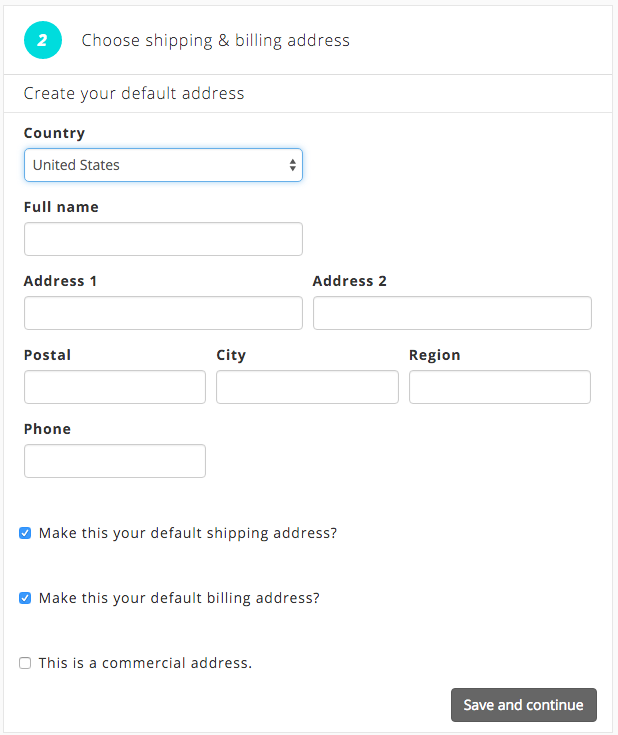
\includegraphics[width=0.6\textwidth]{figuras/shipping/form_address.png}
		\caption{Despliegue automático del formulario de direcciones cuando no se tienen ninguna dirección agregada.}
		\label{figure:checkout:form_address_default}
	\end{figure}